\documentclass[10pt,a4paper]{article}
\usepackage[margin=2.2cm]{geometry}
\usepackage{amsmath,amssymb}
\usepackage{booktabs,tabularx,array}
\usepackage{xcolor}
\usepackage{tikz}
\usetikzlibrary{arrows.meta,positioning}
\usepackage{fancyhdr}
\usepackage{titlesec}
\usepackage{enumitem}
\usepackage[hidelinks]{hyperref}
\usepackage{tcolorbox}

\definecolor{accent}{HTML}{1F4E79}
\definecolor{contrib}{HTML}{FCE9D9}
\definecolor{done}{HTML}{2E7D32}
\definecolor{prog}{HTML}{B26A00}
\definecolor{todo}{HTML}{9E2A2B}

\newcommand{\done}{\textcolor{done}{\textbf{Done}}}
\newcommand{\prog}{\textcolor{prog}{\textbf{In progress}}}
\newcommand{\todo}{\textcolor{todo}{\textbf{To do}}}
\newcommand{\later}{\textcolor{gray}{\textbf{Phase 2}}}

\titleformat{\section}{\large\bfseries\color{accent}}{\thesection}{0.6em}{}
\titleformat{\subsection}{\normalsize\bfseries}{\thesubsection}{0.5em}{}
\setlist{itemsep=1pt,topsep=3pt}

\pagestyle{fancy}
\fancyhf{}
\fancyhead[L]{\small Reliable and Secure ReRAM Crossbar Accelerators}
\fancyhead[R]{\small CS5290 -- Project Plan (rev.\ 2)}
\fancyfoot[C]{\small\thepage}

\newtcolorbox{contribbox}[1]{colback=contrib,colframe=accent,boxrule=0.5pt,arc=1pt,
  left=5pt,right=5pt,top=3pt,bottom=3pt,title={#1},fonttitle=\bfseries\small,coltitle=white}

\begin{document}

\begin{center}
{\small CS5290 Memory-Centric Computer Architecture $\cdot$ Course Project Plan (Revision 2, 23 October 2026)}\\[6pt]
{\LARGE\bfseries Reliable and Secure ReRAM Crossbar Accelerators}\\[2pt]
{\LARGE\bfseries for Deep Neural Networks}\\[6pt]
{\large Noise-, Fault- and Attack-Aware Hybrid SLC/MLC In-Memory Computing}
\end{center}

\noindent\textbf{Abstract.} Resistive RAM (ReRAM) crossbars perform matrix--vector multiplication in
place, removing the weight movement that dominates the energy of deep neural network (DNN) inference.
Their practical use is limited by device non-idealities (conductance variation, stuck-at faults,
limited multi-level precision, ADC quantisation and IR drop) and by the exposure of in-memory weights
to fault-injection attacks. Building on HyFlexPIM, which places important weights in reliable
single-level cells (SLC) and the remainder in dense multi-level cells (MLC), we will (i) develop and
verify a bit-accurate crossbar simulator, (ii) reproduce the key published baselines, (iii)
characterise the impact of each non-ideality, (iv) recover accuracy through noise-aware training,
noise-aware mapping and fault-aware mapping, and (v) propose a \emph{unified rank-to-slot mapping} that
jointly accounts for cell tier, stuck-at faults and IR drop at zero runtime hardware cost. We further
evaluate a multi-level-cell bit-flip attack and an analog checksum defence, and quantify all overheads
with NeuroSim. Work proceeds in two phases: \textbf{Phase~1} takes two Transformers (DistilBERT and
BERT-Base on SST-2) through every step; \textbf{Phase~2} extends the same pipeline to CNNs, to a second
GLUE task (MRPC) and to an FPGA emulator on the AMD Kria KV260.

\vspace{4pt}
\noindent\textbf{Changes from Revision 1.}
(a) Work is split into two phases, Transformers first (Section~5);
(b) DistilBERT is added as a fast development model;
(c) public SST-2 fine-tuned checkpoints replace training from scratch, and the INT8 reference is
post-training quantisation;
(d) all compute runs on \textbf{Kaggle} GPU notebooks;
(e) simulator details now match the implementation (7 SLC / 4 MLC cells per 8-bit weight);
(f) a progress-to-date section is added.

\section{Papers Included in the Project}

The project is anchored on one primary paper, extends four foundational works, and draws on a small
set of recent papers for baselines and techniques (Table~\ref{tab:papers}).

\begin{table}[h]
\centering\small
\caption{Papers included in the project and their role.}\label{tab:papers}
\begin{tabularx}{\linewidth}{@{}l l X@{}}
\toprule
Role & Paper & What we use \\
\midrule
Primary & HyFlexPIM, Song \emph{et al.}, ISCA 2025 & Hybrid SLC/MLC analog PIM; SVD-based gradient redistribution; importance-based tier mapping. Reproduced and extended. \\
Foundational & ISAAC, Shafiee \emph{et al.}, ISCA 2016 & Reference crossbar organisation (tiles, bit-slicing, ADC sharing); PPA baseline. \\
architecture & PRIME, Chi \emph{et al.}, ISCA 2016 & ReRAM main-memory PIM organisation; signed-weight mapping. \\
Reliability & Xia \emph{et al.}, DAC 2017 & Fault-tolerant training and remapping for stuck-at faults; baseline for our mapping. \\
Security & Rakin \emph{et al.}, ICCV 2019 & Bit-Flip Attack (progressive bit search); reproduced on crossbar-stored weights. \\
\midrule
Supporting & Rasch \emph{et al.}, Nat.\ Commun.\ 2023 & Hardware-aware (noise-aware) training baseline. \\
 & Chen \emph{et al.}, DATE 2017 & Optimal (bipartite) fault-aware weight mapping baseline. \\
 & FREEMAP, ISLPED 2026 & Zero-overhead folding of permutations into adjacent layers. \\
 & SWIM, DAC 2022 & Hessian-based weight-importance metric. \\
 & Liu \emph{et al.}, ITC 2018; RADAR, DATE 2021 & Checksum-based error and attack detection. \\
 & Luo \emph{et al.}, TCAD 2020 & FPGA emulation of ReRAM crossbars with noise. \\
\bottomrule
\end{tabularx}
\end{table}

\section{Project Overview}

\textbf{Problem.} A ReRAM crossbar stores weights as conductances $G_{ij}$; applying input voltages
$V_i$ to the rows yields column currents $I_j=\sum_i V_i G_{ij}$, i.e.\ an analog dot product. Real
devices deviate from their programmed values, some cells are permanently stuck, multi-level cells have
narrow noise margins, and wire resistance attenuates currents. Because weights reside in memory, an
adversary able to perturb a few cells can also collapse model accuracy.

\textbf{Gap in the primary paper.} HyFlexPIM models device noise only as i.i.d.\ multiplicative
Gaussian weight noise; it does not consider stuck-at faults, IR drop or drift, applies no noise-aware
training, ignores \emph{which physical cells} hold a given weight, provides no security analysis, and is
evaluated on Transformers only.

\textbf{Objectives.}
\begin{description}[leftmargin=2.2em,labelwidth=1.8em,font=\normalfont\bfseries]
\item[O1] Build a bit-accurate, verified ReRAM crossbar simulator and reproduce published baselines.
\item[O2] Characterise the accuracy impact of each non-ideality, individually and combined.
\item[O3] Recover accuracy via noise-aware training, noise-aware mapping and fault-aware mapping.
\item[O4] Secure crossbar-stored weights against bit-flip attacks at low overhead.
\item[O5] Quantify the energy, latency and area cost of every technique; demonstrate an FPGA emulator (Phase 2).
\end{description}

\textbf{Planned contributions.}
\begin{description}[leftmargin=2.2em,labelwidth=1.8em,font=\normalfont\bfseries]
\item[C1] \emph{Unified rank-to-slot mapping.} A single optimal assignment that places each SVD
component in a physical crossbar slot, jointly considering cell tier (SLC/MLC), stuck-at faults and
IR-drop position, with no runtime permutation hardware.
\item[C2] \emph{Tier-aware noise-aware training.} Fine-tuning with SLC-level noise on protected
components and MLC-level noise elsewhere, to reduce the required SLC fraction.
\item[C3] \emph{Multi-level-cell bit-flip threat model.} Attack cost measured in conductance-level
shifts rather than bit flips, and the effect of level encoding (binary vs.\ Gray).
\item[C4] \emph{Analog checksum defence.} A per-crossbar checksum column evaluated against benign
noise (false alarms) and an adaptive, checksum-aware attacker.
\end{description}

\textbf{Scope.} One simulator serves all models.
\begin{itemize}
\item \textbf{Phase 1 -- Transformer track (current):} DistilBERT (36 encoder linear layers) and
BERT-Base (72 layers) on GLUE SST-2, for direct comparison with HyFlexPIM. DistilBERT is the fast
development model; BERT-Base is the reported result.
\item \textbf{Phase 2 -- Extension:} BERT-Base on GLUE MRPC; a CNN track (ResNet-20, ResNet-18, VGG-16 on
CIFAR-10); KV260 FPGA emulation with ResNet-20.
\end{itemize}

\begin{figure}[h]
\centering
\resizebox{\linewidth}{!}{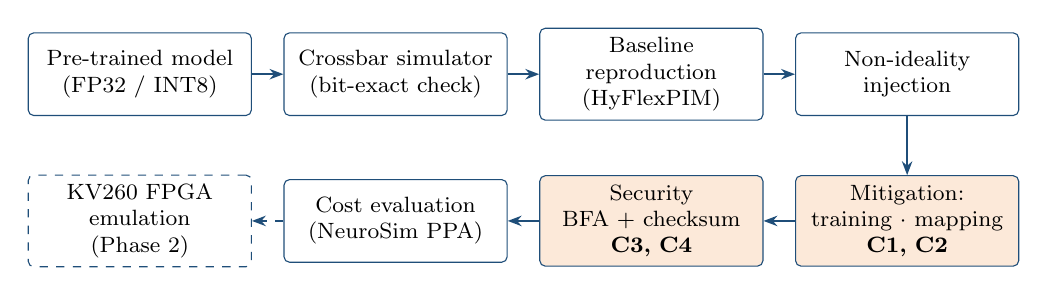
\begin{tikzpicture}[
  box/.style={draw=accent,rounded corners=2pt,align=center,font=\footnotesize,minimum height=1.05cm,text width=2.6cm,fill=white},
  hl/.style={box,fill=contrib},
  arr/.style={-{Stealth[length=5pt]},accent,thick},
  node distance=0.4cm,scale=1]
\node[box] (a) {Pre-trained model\\(FP32 / INT8)};
\node[box,right=of a] (b) {Crossbar simulator\\(bit-exact check)};
\node[box,right=of b] (c) {Baseline\\reproduction\\(HyFlexPIM)};
\node[box,right=of c] (d) {Non-ideality\\injection};
\node[hl,below=0.75cm of d] (e) {Mitigation:\\training $\cdot$ mapping\\\textbf{C1, C2}};
\node[hl,left=of e] (f) {Security\\BFA + checksum\\\textbf{C3, C4}};
\node[box,left=of f] (g) {Cost evaluation\\(NeuroSim PPA)};
\node[box,left=of g,dashed] (h) {KV260 FPGA\\emulation\\(Phase 2)};
\draw[arr] (a)--(b); \draw[arr] (b)--(c); \draw[arr] (c)--(d); \draw[arr] (d)--(e);
\draw[arr] (e)--(f); \draw[arr] (f)--(g); \draw[arr,dashed] (g)--(h);
\end{tikzpicture}}
\caption{Project workflow. Shaded stages contain our contributions; dashed stage is Phase 2.}
\end{figure}

\section{Methodology}

\subsection{Step 1 -- Baseline Models and Quantisation}
\textbf{Phase 1.} We use public checkpoints already fine-tuned on SST-2 from Hugging Face, so no training
from scratch is needed:
\begin{itemize}
\item DistilBERT: \texttt{distilbert-base-uncased-finetuned-sst-2-english}
\item BERT-Base: \texttt{textattack/bert-base-uncased-SST-2}
\end{itemize} We report two
references on the 872-sentence SST-2 validation set:
(i) \emph{FP32 accuracy} of the unmodified model, and
(ii) \emph{INT8 accuracy}: weights quantised with symmetric per-output-channel 8-bit scales and
activations with an 8-bit per-tensor scale (post-training quantisation, no noise, no SVD).
These are the accuracy references for all later steps.

\textbf{Phase 2.} FP32 baselines for ResNet-20, ResNet-18 and VGG-16 on CIFAR-10 are trained on Kaggle,
followed by INT8 quantisation-aware training; BERT-Base on MRPC uses a public fine-tuned checkpoint.

\subsection{Step 2 -- Bit-Accurate Crossbar Simulator}
We implement a PyTorch library (\texttt{reram\_sim}) in which every target linear layer (and, in
Phase 2, every convolution via im2col) is replaced by a crossbar layer that models the analog
computation explicitly:
\begin{itemize}
\item \textbf{Quantisation and signed weights.} Each weight row is quantised to a signed 8-bit integer
$q\in[-127,127]$ and stored as a differential pair, $q=q^{+}-q^{-}$, $w_{ij}\propto G^{+}_{ij}-G^{-}_{ij}$.
\item \textbf{Bit-slicing.} The 7-bit magnitude is split into base-$2^b$ digits,
$q^{\pm}=\sum_s 2^{sb}\,d^{(s)}$, with $b=1$ (SLC, 7 cells) or $b=2$ (MLC, 4 cells), tiled into
$128\times128$ arrays.
\item \textbf{Conductance levels.} Digit $d$ is programmed as $G=G_{\min}+d\,\Delta$,
$\Delta=(G_{\max}-G_{\min})/(2^b-1)$, with $G_{\max}=1$ (normalised) and $G_{\max}/G_{\min}=100$. MLC
levels are therefore $3\times$ closer than SLC levels.
\item \textbf{Inputs, ADC and shift-and-add.} Inputs are quantised to 8 bits by the DAC; each slice
and 128-row tile is read by an ADC and combined digitally:
\begin{equation}
y_j=\sum_t\sum_s 2^{\,t+sb}\,\mathrm{ADC}\!\Big(\sum_i x_i^{(t)} w_{ij}^{(s)}\Big),
\end{equation}
where $x_i^{(t)}$ is the $t$-th input bit. The current implementation applies whole 8-bit inputs and
a batch-calibrated ADC; bit-serial inputs and a fixed (offline-calibrated) ADC range are added in this
step.
\item \textbf{Chips.} One seeded random generator programs a whole model; each seed is one simulated chip.
\end{itemize}

\textbf{Verification.} With all non-idealities disabled and a lossless ADC of
$b_{\mathrm{ADC}}=\lceil\log_2(R(2^b-1)+1)\rceil$ bits ($R$ rows), the simulator must reproduce the INT8
model exactly on every layer and in end-to-end accuracy. Automated tests (16 so far: toy matrices, a toy
MLP, a Transformer encoder layer and DistilBERT end-to-end) are re-run after every change.

\subsection{Step 3 -- Reproduction of Baselines}
\begin{itemize}
\item \textbf{HyFlexPIM method.} Our re-implementation: every encoder linear layer is factorised as
$W\approx U_k\Sigma_k V_k^{\top}$ with the parameter-preserving rank $k=\lfloor mn/(m+n)\rfloor$
(e.g.\ $k=384$ for $768\times768$), fine-tuned on SST-2 (8 epochs, AdamW, lr $2\times10^{-5}$) to
recover truncation loss, and scored by $I_r=|\partial L/\partial\sigma_r|$ over 2048 calibration
sentences. The top 20\% of components per layer are placed in SLC, the rest in MLC; on hardware each
tier is two crossbars back to back, \[y=U_{\mathrm{SLC}}(\Sigma V^{\top})_{\mathrm{SLC}}\,x+U_{\mathrm{MLC}}(\Sigma V^{\top})_{\mathrm{MLC}}\,x+b.\]
\item \textbf{HyFlexPIM results.} Accuracy versus noise for five placement policies (all-SLC, all-MLC,
gradient, magnitude, random) and accuracy versus SLC fraction (0--100\%). Expected: gradient placement
stays close to all-SLC at 20\% SLC. Results are cross-checked against the authors' open-source code.
\item \textbf{ISAAC/PRIME-style PPA.} NeuroSim V1.5 energy, latency, area, TOPS/W and ADC energy share,
against a digital baseline (Step 6).
\item \textbf{Bit-Flip Attack.} The attack of Rakin \emph{et al.} reproduced on the 8-bit weights of
BERT-Base and DistilBERT, recording flips needed to reach random-guess accuracy (50\%) (Step 7).
\item \textbf{Phase 2.} HyFlexPIM on CNNs: whether importance concentrates in few components, as it does
for Transformers.
\end{itemize}

\subsection{Step 4 -- Non-Ideality Modelling and Characterisation}
Each effect is an independent, seeded module (Table~\ref{tab:noise}). Parameters are taken from
measured ReRAM data in the literature and the noise models of IBM AIHWKIT; the simulator is
cross-checked against AIHWKIT and, for IR drop, Sandia CrossSim. Initial sweeps use 5 chips per point;
final results use at least 20 chips, reporting mean, 5th-percentile and worst-case accuracy, together with
a per-layer sensitivity analysis.

\begin{table}[h]
\centering\small
\caption{Modelled non-idealities.}\label{tab:noise}
\begin{tabularx}{\linewidth}{@{}l X l l@{}}
\toprule
Effect & Model & Sweep & Status \\
\midrule
Programming variation & $\tilde G=G+\sigma G_{\max}\,\mathcal N(0,1)$, fixed per chip; same $\sigma$ hurts MLC more & $\sigma\in[0,10]\%$ & Implemented \\
Read noise & Fresh Gaussian perturbation at every inference & 0.5--2\% & To add \\
Stuck-at faults (uniform) & Cell forced to $G_{\max}$ or $G_{\min}$ with probability $p$ & 0.1--20\% of cells & Implemented \\
Stuck-at faults (clustered) & Whole rows / columns dead & 0.1--5\% of lines & To add \\
Limited levels & 1 or 2 bits/cell; smaller level margin for MLC & SLC vs.\ MLC & Implemented \\
ADC resolution & Clamp and round of column partial sums per tile & 3--8 bits & Implemented \\
IR drop & Position-dependent attenuation along word/bit lines & $r_{\mathrm{wire}}\times$ size (64--256) & To add \\
Drift (optional) & Time-dependent conductance relaxation & 1\,s to 1 week & Optional \\
\bottomrule
\end{tabularx}
\end{table}

\subsection{Step 5 -- Accuracy Recovery}
\textbf{5a. Noise-aware training (NAT).} We train
$\min_\theta \mathbb E_\eta\big[L(f(x;\theta\odot(1+\eta)))\big]$, resampling noise every mini-batch with
straight-through quantisation. Methods are evaluated incrementally: (i) Gaussian noise injection;
(ii) the hardware-aware training recipe of Rasch \emph{et al.} via AIHWKIT; (iii) stuck-at fault injection
during training; (iv) worst-case-oriented objectives.

\textbf{5b. SVD and noise-aware mapping.} Starting from the Step 3 tiering, we compare gradient,
magnitude, Hessian (SWIM) and Fisher importance at the component and layer level, and select per-layer
SLC fractions under a NeuroSim area/energy budget.

\begin{contribbox}{Contribution C2 -- Tier-aware noise-aware training}
During the HyFlexPIM fine-tune, components currently assigned to SLC receive SLC-level noise and the
remaining components MLC-level noise, $\eta_r\sim\mathcal N(0,\sigma^2_{\tau(r)})$, with the assignment
$\tau$ refreshed periodically. The network learns to concentrate information where it is protected.
\emph{Hypothesis:} equal accuracy at a lower SLC fraction.
\end{contribbox}

\textbf{5c. Fault-aware mapping.} Given a chip's stuck-at fault map, logical rows are assigned to
physical rows by solving the linear assignment problem
\begin{equation}
\pi^\star=\arg\min_\pi\sum_i C_{i,\pi(i)},\qquad C_{ij}=\sum_k I_{ik}\big(w_{ik}-\hat w^{(j)}_{ik}\big)^2,
\end{equation}
where $\hat w^{(j)}_{ik}$ is the value realised when row $i$ is stored on physical row $j$. It is solved
optimally with the Hungarian algorithm (\texttt{scipy.optimize.linear\_sum\_assignment}); row and column
permutations are alternated. Output-column permutations are folded into the next layer's input order (as
in FREEMAP), so no permutation hardware is required. Spare rows, allocated by importance, handle
clustered faults. Baselines: no mitigation, Xia \emph{et al.}, Chen \emph{et al.} and fault-injection
training.

\begin{contribbox}{Contribution C1 -- Unified rank-to-slot mapping}
In an SVD-factorised layer $W=U(\Sigma V^{\top})$ the $k$ components form an internal dimension that can be
permuted (columns of $U$ and rows of $\Sigma V^{\top}$ together) without changing the layer output. Each
physical slot $s$ is characterised by its tier $\tau(s)\in\{\mathrm{SLC},\mathrm{MLC}\}$, its fault
pattern $F_s$ and its IR-drop attenuation $\alpha_s$. We solve
\[
\min_\pi\sum_r I_r\,\mathbb E\big[\|\Delta_r(\pi(r))\|^2\,\big|\,\tau,F,\alpha\big]\quad
\text{s.t. SLC capacity budget,}
\]
unifying tier allocation (HyFlexPIM), fault-aware remapping and IR-drop-aware placement in a single optimal
assignment with zero runtime hardware overhead. An ablation isolates each cost term.
\end{contribbox}

\textbf{5d. Complementary techniques (time permitting).} Drift compensation, sign-flip weight storage
matched to fault patterns, activation clipping, and reduced ADC precision for MLC arrays.

\subsection{Step 6 -- Hardware Cost Evaluation}
All configurations are evaluated in NeuroSim V1.5 (Transformers; Phase 1) and DNN+NeuroSim V1.4 (CNNs;
Phase 2) for energy per inference, latency, area, TOPS/W and TOPS/mm$^2$, with an energy breakdown (ADC,
array, peripherals, buffers). The overhead of each technique (additional SLC cells, spare rows, checksum
columns) is reported. The central result is the \emph{accuracy--efficiency Pareto front} obtained by
varying the SLC fraction.

\subsection{Step 7 -- Security}
\textbf{Threat model.} The adversary shifts cell conductance levels through physical disturbance
(thermal crosstalk, write or read disturbance), restricted to cells physically reachable from the
attacker's access pattern.

\begin{contribbox}{Contributions C3 and C4 -- MLC-aware attack and analog checksum defence}
\textbf{C3.} The Bit-Flip Attack is reformulated with cost measured in conductance-level shifts: in a
2-bit cell one shift may flip two bits. We test whether MLC lowers attack cost and whether Gray-coded
levels remove this advantage.\\[2pt]
\textbf{C4.} Each crossbar holds a checksum column $G_{i,\mathrm{chk}}=\sum_j G_{ij}$; tampering is
flagged when $\big|\sum_j I_j-I_{\mathrm{chk}}\big|>\theta$, with $\theta$ set from the benign-noise
distribution (cost $\approx1/128$ columns). Unlike prior checksum schemes for random faults (X-ABFT) or
digital weights (RADAR), we evaluate against an adaptive attacker that preserves the checksum, countered
by a secret-weighted checksum.
\end{contribbox}

\textbf{Evaluation:} flips or level shifts required to reach random-guess accuracy, with and without
each defence (noise-aware training, SLC protection, Gray coding, checksum); detection ROC and AUC;
detection latency; recovery by row reprogramming.

\subsection{Step 8 -- FPGA Emulation on AMD Kria KV260 (Phase 2)}
The emulator implements the arithmetic of the simulator exactly, so that the simulator serves as its
golden model. BERT-Base does not fit on-chip, so the emulator targets ResNet-20 (0.27\,M weights).
\begin{itemize}
\item \textbf{Processing system (ARM, PYNQ):} loads conductance codes and stuck-at masks, configures ADC
precision and noise level through AXI-Lite, and streams activations via DMA.
\item \textbf{Programmable logic (Vitis HLS):} several $128\times128$ virtual-crossbar tiles, each with
on-chip weight storage, parallel MAC lanes, hardware Gaussian noise generators (Tausworthe-based,
following Luo \emph{et al.}), ADC rounding, shift-and-add and an optional checksum column.
\item \textbf{Mapping:} fault-aware and rank permutations are folded into the stored weights and need
no logic, demonstrating C1's zero-overhead property.
\item \textbf{Validation:} bit-exact agreement with noise disabled, statistical agreement with noise
enabled, speed-up over the software simulator, resource utilisation, clock frequency and board power.
\end{itemize}

\section{Tools and Frameworks}

\begin{table}[h]
\centering\small
\caption{Software and hardware tools.}
\begin{tabularx}{\linewidth}{@{}l l X@{}}
\toprule
Purpose & Tool & Role in the project \\
\midrule
Core simulation & Custom PyTorch library & Crossbar model, non-idealities, SLC/MLC tiers, mappings; FPGA golden model \\
Models and data & Hugging Face \texttt{transformers}, \texttt{datasets} & Pre-trained checkpoints; GLUE SST-2 (and MRPC) \\
Analog reference & IBM AIHWKIT & Calibrated ReRAM noise models, simulator validation, NAT baseline \\
IR-drop validation & Sandia CrossSim & Circuit-level parasitic solver \\
Primary baseline & HyFlexPIM code & Cross-check of our SVD and tiering pipeline \\
Energy, latency, area & NeuroSim V1.5 / DNN+NeuroSim V1.4 & PPA of all configurations \\
Optimisation & SciPy, PuLP / OR-Tools & Hungarian assignment and ILP \\
Security & Public BFA implementation & Attack reproduction and extension \\
FPGA (Phase 2) & Vitis HLS, Vivado, Kria-PYNQ & KV260 emulator (Linux x86 host required) \\
Compute & \textbf{Kaggle} notebooks (NVIDIA T4 GPU), laptops & All training and Monte Carlo sweeps run as Kaggle notebooks (30 GPU-h/week, 12\,h sessions); laptops for development and unit tests only \\
\bottomrule
\end{tabularx}
\end{table}

\section{Execution Order and Progress}

\subsection{Phase 1 -- DistilBERT and BERT-Base on SST-2}
Tasks run in this order; each uses the output of the previous one.

\begin{table}[h]
\centering\small
\begin{tabularx}{\linewidth}{@{}c l X l@{}}
\toprule
\# & Plan step & Task & Status \\
\midrule
1 & Step 1 & FP32 accuracy of both pre-trained models & \done \\
2 & Step 1 & INT8 (post-training) accuracy of both models & \done \\
3 & Step 3 & HyFlexPIM pipeline: SVD, fine-tune, gradient importance, 20\% SLC split & \done \\
4 & Step 2 & Crossbar simulator (quantise, differential pair, bit-slice, noise, faults, DAC/ADC) + 16 tests & \done \\
5 & Step 2 & End-to-end check: simulator at $\sigma=0$ matches the SVD model & \done \\
6 & Step 3 & Five placement policies vs.\ programming noise ($\sigma=0$--10\%) & \done \\
7 & Step 3 & Accuracy vs.\ SLC fraction (0, 5, 10, 20, 30, 50, 100\%) for gradient, magnitude, random and Fisher importance (Fisher brought forward from Step 5b), $\sigma=3,5,7.5\%$, 20 chips & \done \\
8 & Step 4 & Stuck-at fault sweep (0--5\% of cells, half stuck at $G_{\max}$, half at $G_{\min}$) for all six placements, 20 chips & \todo\ (script ready) \\
9 & Step 2/4 & Add bit-serial inputs, fixed calibrated ADC (then ADC-bits sweep, 3--8 bits), read noise, clustered faults, IR drop; 20 chips & \todo \\
10 & Step 5a & Noise-aware training & \todo \\
11 & Step 5b & \textbf{C2} tier-aware noise-aware training & \todo \\
12 & Step 5c & Fault-aware mapping (Hungarian) & \todo \\
13 & Step 5c & \textbf{C1} unified rank-to-slot mapping & \todo \\
14 & Step 7 & Bit-Flip Attack, \textbf{C3}, \textbf{C4} & \todo \\
15 & Step 6 & NeuroSim V1.5 PPA and accuracy--efficiency Pareto front & \todo \\
\bottomrule
\end{tabularx}
\end{table}

\subsection{Phase 2 -- Extension}
(16) BERT-Base on MRPC; (17) CNN track: ResNet-20/18 and VGG-16 on CIFAR-10 with QAT, conv layers via
im2col, repeat tasks 5--15; (18) KV260 FPGA emulator with ResNet-20.

\subsection{Results to Date}
\textbf{Tasks 1--3.} Kaggle T4, 8 fine-tuning epochs, 20\% SLC per layer. The SLC and MLC parts sum back
to the factorised weight with a maximum absolute error below $4\times10^{-6}$. INT8 is the original
(non-SVD) model with its encoder layers quantised to 8 bits.

\begin{table}[h]
\centering\small
\begin{tabular}{@{}lccccc@{}}
\toprule
Model & FP32 & INT8 & SVD truncated & SVD + fine-tune & Components in SLC \\
\midrule
DistilBERT (36 layers) & 91.06\% & 90.37\% & 89.68\% & 89.11\% & 3{,}324 / 16{,}584 (20.0\%) \\
BERT-Base (72 layers) & 92.43\% & 91.86\% & 89.33\% & 90.14\% & 6{,}648 / 33{,}168 (20.0\%) \\
\bottomrule
\end{tabular}
\end{table}

\noindent\textbf{Tasks 5--6.} With no noise ($\sigma=0$) the BERT-Base crossbar model reaches
89.7--90.3\% for every placement, within 0.5 points of the digital SVD model (task 5). Table below:
mean SST-2 accuracy of BERT-Base over 5 simulated chips versus programming noise (task 6).

\begin{table}[h]
\centering\small
\begin{tabular}{@{}lcccccc@{}}
\toprule
Placement & $\sigma=0$ & 2\% & 3\% & 5\% & 7.5\% & 10\% \\
\midrule
All SLC & 89.9 & 89.3 & 89.1 & 87.8 & 85.9 & 79.7 \\
All MLC & 90.0 & 87.3 & 83.9 & 66.3 & 52.2 & 51.3 \\
Gradient, 20\% SLC (HyFlexPIM) & 90.3 & 89.7 & 89.5 & 85.8 & 72.1 & 60.3 \\
Magnitude, 20\% SLC & 89.7 & 89.9 & 90.0 & 88.6 & 83.5 & 72.0 \\
Random, 20\% SLC & 90.0 & 89.9 & 87.7 & 78.8 & 58.8 & 49.1 \\
\bottomrule
\end{tabular}
\end{table}

\noindent All-MLC collapses to near random guessing for $\sigma\geq5\%$, and protecting 20\% of
components recovers most of the loss, so the choice of components matters (random is far worse).
Unexpectedly, \emph{magnitude} selection outperforms HyFlexPIM's \emph{gradient} selection for
$\sigma\geq5\%$, on DistilBERT as well.

\noindent\textbf{Task 7.} Mean SST-2 accuracy of BERT-Base over 20 simulated chips versus the fraction of
components stored in SLC (same fine-tuned SVD model; only the SLC/MLC assignment changes).
All-MLC (0\%) and all-SLC (100\%) are shown for reference.

\begin{table}[h]
\centering\small
\begin{tabular}{@{}llccccccc@{}}
\toprule
$\sigma$ & Policy & 0\% & 5\% & 10\% & 20\% & 30\% & 50\% & 100\% \\
\midrule
5\%   & Gradient  & 66.8 & 83.0 & 82.0 & 86.5 & 86.1 & 88.1 & 88.0 \\
      & Fisher    &      & 87.3 & 87.9 & 88.1 & 88.3 & 88.4 & \\
      & Magnitude &      & 88.0 & 88.6 & 88.7 & 88.9 & 88.9 & \\
      & Random    &      & 72.5 & 73.6 & 76.2 & 77.8 & 83.4 & \\
\midrule
7.5\% & Gradient  & 53.0 & 66.2 & 62.9 & 73.0 & 73.9 & 79.6 & 85.7 \\
      & Fisher    &      & 75.6 & 78.9 & 80.3 & 82.2 & 83.8 & \\
      & Magnitude &      & 79.4 & 81.8 & 84.1 & 85.5 & 85.6 & \\
      & Random    &      & 53.6 & 54.2 & 55.2 & 57.5 & 67.3 & \\
\bottomrule
\end{tabular}
\end{table}

\noindent Findings (DistilBERT shows the same ordering): (a) the ranking is
magnitude $>$ Fisher $>$ gradient $\gg$ random at every SLC fraction, and magnitude also has the best
worst-chip accuracy; (b) Fisher, which squares per-sentence gradients and so cannot cancel, closes most
of the gap between gradient and magnitude, so sign cancellation explains part of the gradient method's
weakness but not all of it; (c) with magnitude selection, 5--10\% SLC is enough at $\sigma=5\%$ and
30\% at $\sigma=7.5\%$ to come within 0.5 points of all-SLC, while gradient needs 50\%; (d) at
$\sigma=3\%$ every importance-based policy is within 1 point of all-SLC even at 5\% SLC.

\noindent\textbf{Open issues.} (i) The SVD loss (2.3 points for BERT-Base) will be compared with the
accuracy reported by HyFlexPIM, and the fine-tuning schedule revisited if the gap is larger. (ii) For
DistilBERT, fine-tuning slightly reduced accuracy, suggesting over-fitting; validation-based early
stopping will be added. (iii) Hypothesis for the remaining magnitude--Fisher gap (to be tested):
programming noise is a fixed fraction of $G_{\max}$, so the large-$\sigma_r$ components carry the most
absolute error. Magnitude selection is used as the default policy from task 8 onwards, with gradient
kept as the HyFlexPIM baseline.

\end{document}
